
\section{\textcolor{black}{Inverse uncertainty}}
%----------------------------------------------
\subsection{Uncertainty to be considered}

%-----------------------------------------------------------------------------------
\begin{frame}
\frametitle{Choice for UQ inversion}
\begin{columns}
    \column{0.5\textwidth}
        Choice for the UQ method is totally based on the {\textcolor{red}{\textbf{quantity}}} of accessible data:
        \begin{itemize}
            \item  {\textcolor{red}{\textbf{Lack}}} or {\textcolor{red}{\textbf{no}}} data available, model can be solely based on expert judgement
            \item {\textcolor{red}{\textbf{Substantial}}} volume data available, model can fully use statistical inference (e.g., the methods of moments)
            \item {\textcolor{red}{\textbf{Combination}}} of two above: Bayesian methods
            \begin{equation*}           \pi(\boldsymbol{x}|\mathcal{Y}) = \frac{{\mathcal{L}(\boldsymbol{x}|\mathcal{Y}) \cdot \pi(\boldsymbol{x})}}{{\pi(\mathcal{Y})}} 
            \end{equation*}
        \end{itemize}
    
    \column{0.5\textwidth}
        \begin{figure}[!ht]       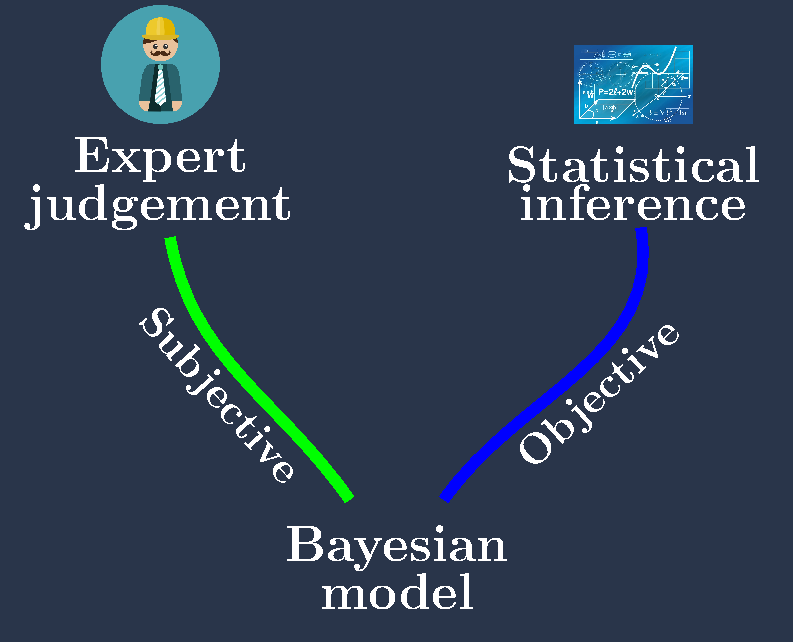
\includegraphics[scale=0.6]{figures/figure_objvssub.pdf}
        \end{figure}
\end{columns}
    
\end{frame}
%===================================================================================================================
\begin{frame}
\frametitle{Posing the probabilistic problem}
\begin{block}{Uncertainties in math form:}
\begin{equation*}
\mathcal{Y}_i = \tilde{\mathcal{M}}(\boldsymbol{x}_i,\boldsymbol{\theta}^{\star}) 
+ \delta(\boldsymbol{x}_i)+
\boldsymbol{\epsilon}_{i}, i=1,\cdots,N
\end{equation*}
$\mathcal{Y}_i$: observation; $\boldsymbol{x}_i$: control inputs; $\boldsymbol{\theta}^{\star}$: true value of calibrated parameters; $\tilde{\mathcal{M}}$: forward model; $\delta$: model discrepancy; $\boldsymbol{\epsilon}_{i}$: observation error  
\end{block}

\begin{block}{Three speficic types of uncertainties (mixed with aleatoric and epistemic): }
\begin{itemize}
    \item observation error
    \item model discrepancy
    \item input space uncertainties
\end{itemize}    
\end{block}

\begin{alertblock}{Should we consider aleatoric uncertainty (irreducible) in the inversion process?}
\begin{itemize}
    \item Or all burden will be shared by other epistemic uncertainty \alert{unreasonably}
\end{itemize}
    
\end{alertblock}
 
\end{frame}







%--------------------------------------------------------------------------------
\subsection{How likelihood dealing with uncertainties?}
\begin{frame}
    

\begin{block}{If only consider a Gaussian type observation error}
\begin{equation*}
\mathcal{Y}_i = \tilde{\mathcal{M}}(\boldsymbol{x}_i,\boldsymbol{\theta}^{\star}) +\boldsymbol{\epsilon}_{i}, i=1,\cdots,N
\end{equation*}
\begin{equation*}        
        \label{eq: Likelihood function}
        \begin{aligned}
         \mathcal{L}(\boldsymbol{\theta}|\mathcal{Y}) =& \prod_{i=1}^{N} N(\mathcal{Y}_{i}|\tilde{\mathcal{M}}(\boldsymbol{x}_i,\boldsymbol{\theta}),\boldsymbol{\Sigma}) \\
         =& \prod_{i=1}^{N}\frac{1}{\sqrt{(2 \pi)^{N_{\rm{out}}}{\rm{det}}         (\boldsymbol{\Sigma})}}\exp\left(-\frac{1}{2}\left(\mathcal{Y}_{i} - \tilde{\mathcal{M}}(\boldsymbol{x}_i,\boldsymbol{\theta})\right)^{\mathsf{T}} \boldsymbol{\Sigma}^{-1}\left(\mathcal{Y}_{i} - \tilde{\mathcal{M}}(\boldsymbol{x}_i,\boldsymbol{\theta})\right)\right) 
        \end{aligned}
        \end{equation*}  
\end{block}

\begin{alertblock}{In real life, only one source of uncertainty is not convincing enough}
\begin{figure}[!ht]       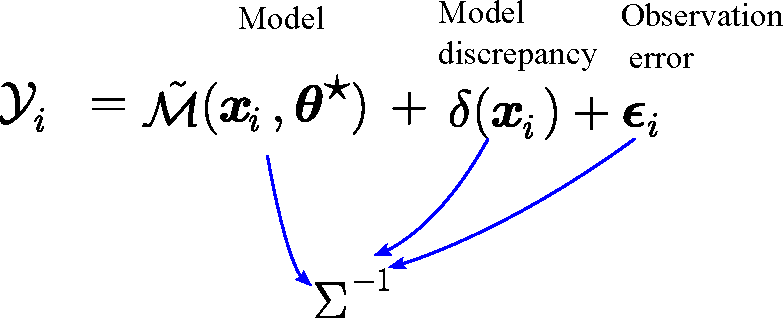
\includegraphics[scale=0.55]{figures/figure-CoVUncertainty.pdf}
\end{figure}
    
\end{alertblock}


\end{frame}
%--------------------------------------------------------------------------------
\begin{frame}
\frametitle{Bayesian inference}
\begin{block}{Difficulty with calculating evidence $\pi(\mathcal{Y})$}
\begin{equation*}               \pi(\boldsymbol{x}|\mathcal{Y}) = 
\frac{{\mathcal{L}(\boldsymbol{x}|\mathcal{Y}) \cdot \pi(\boldsymbol{x})}}{{\pi(\mathcal{Y})}}
= \frac{{\mathcal{L}(\boldsymbol{x}|\mathcal{Y}) \cdot \pi(\boldsymbol{x})}}
{\int_{\mathcal{D}_{\boldsymbol{X}}} 
    \pi(\boldsymbol{x}) \pi(\mathcal{Y}|\boldsymbol{x}) {\rm{d}} \boldsymbol{x}}
\end{equation*}  
\end{block}

Computing evidence ${\pi(\mathcal{Y})}$ is not a tractable problem. A common strategy is using \textit{conjugate priors}  
\begin{itemize}
    \item static Bayesian network
    \item variant elimintion/ belief propagation
    \item kalman filtering
\end{itemize}

\begin{block}{Computational methods:}
 \begin{equation*}               \pi(\boldsymbol{x}|\mathcal{Y}) \approx 
{\mathcal{L}(\boldsymbol{x}|\mathcal{Y}) \cdot \pi(\boldsymbol{x})}
\end{equation*}     
\end{block}
Samples from the posterior can be obtained through \textit{Sampling methods} or \textit{Optimization methods}
\end{frame}
%-------------------------------------------------------------------------------------------
\subsection{Sampling methods}
\begin{frame}
\only<1>{
\begin{definition}
\textbf{Optimisation based approximation}: This method usually refers to variational inference. The basic principle is adopting some analytical distributions to approximate the posterior based on some loss functions
\end{definition}

\begin{block}{PROS and CONS:}
 \begin{itemize}
     \item[\scalebox{1.5} {\color{green}\checkmark}] computational efficient and work well with large model
     \item[\scalebox{1.5} {\color{green}\checkmark}] has absolute converging criteria which makes easy t odetermine when to stop
     \item[\scalebox{1.5}{\color{red}$\times$}] unlikely to discover the globally optimal solution
     \item[\scalebox{1.5}{\color{red}$\times$}] precision constrained by the structure of approximaiton
     
 \end{itemize}   
\end{block}
}


\only<2>{
\begin{definition}
\textbf{Monte Carlo sampling}: These techniques produce random samples from a proposal distribution, utilizing
them to estimate both the posterior distribution and the associated statistics
\end{definition}

Some are:
\begin{itemize}
    \item probability density tranform
    \item rejection sampling
    \item importance sampling
    \item sequential Monte Carlo (e.g., particle filtering)
    \item Markov Chain Monte Carlo (MH, HMC, AIES)
\end{itemize}

}

    
\end{frame}



%------------------------------------------------------------------------------------
\begin{frame}
\frametitle{SMC vs MCMC}
\only<1>{
\begin{quote}
    ... non-iterative methods for generating independent
samples..., we discuss an iterative method known as Markov Chain Monte
Carlo, or \alert{MCMC} for short, which produces dependent samples but \alert{which works well in high
dimensions}...\footfullcite{murphy2012}
\end{quote}


}

\only<2>{

\begin{columns}
    \column{0.45\textwidth}
    \begin{block}{SMC} \animategraphics[autoplay,loop,width=\textwidth]{1}{figures-gif/PF/particlefilter-}{0}{12}        
    \end{block}
    Source:\hyperlink{https://medium.com/@mathiasmantelli/particle-filter-part-3-motion-and-measurement-models-be79857a5490}{weblink}
    \column{0.45\textwidth}
     \begin{block}{MCMC} \animategraphics[autoplay,loop,width=\textwidth]{1}{figures-gif/MCMC/MCMC-}{1}{26}        
    \end{block} 
    Source:\hyperlink{https://www.cdslab.org/DSP2019F/announcement/0-student-professor-connection-day}{weblink}
\end{columns}

}

\end{frame}

